\section{Related Works and Research}
Prior to developing a concept, 
research was done into the topic of monitoring car crashes,
to get inspiration for possible features 
and an understanding of the possible problems in such a project.
\\
\newline
In 2019, researchers from the COMSATS University in Pakistan\cite{iotAccidentSensNRep} 
worked on a similar project. 
They also wanted to improve the response time of emergency vehicles
and looked at a lot of different existing methods of detecting a car crash.
What they found was that a most systems were either lacking in features,
accuracy and reliability or were really expensive.\cite{iotAccidentSensNRep}
\\
\newline
So they proposed a new architecture, 
in the form of an app that runs on the drives smartphone.
This meant that the end cost for the user was basically zero,
provided that they own a compatible smartphone, 
as they also planned to release the app for free.\cite{iotAccidentSensNRep}
The general concept of this architecture can be seen in Figure \ref{6fig:iotArch}.

\begin{figure}[H]
  \centering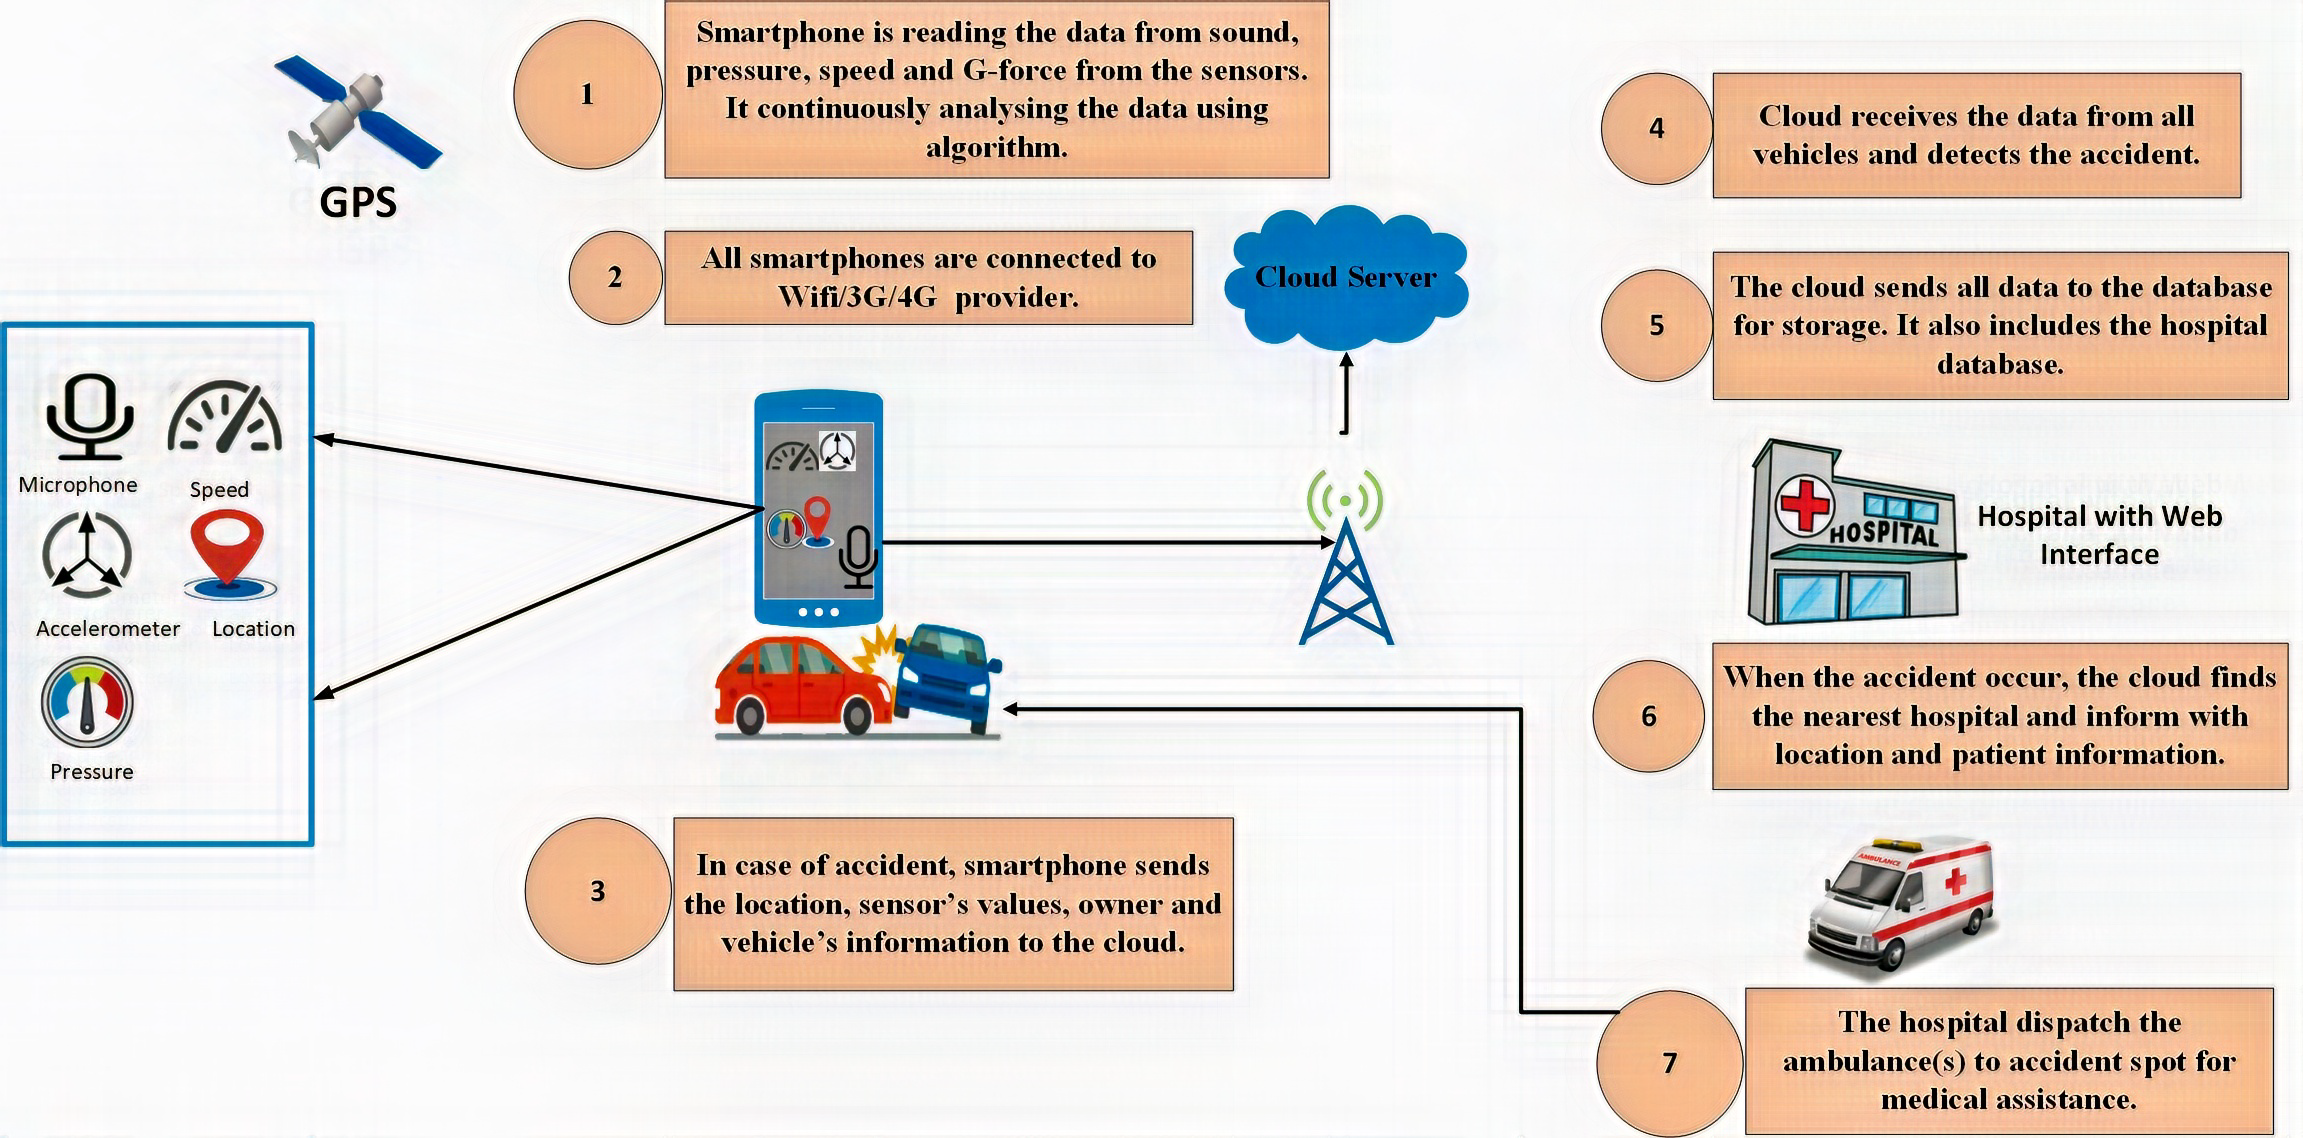
\includegraphics[width=\linewidth]{chapters/chapter6_bruno/Figures/bhattiArticleAbb1.png}
  \caption{Smart City Crash Detection Architecture \cite{iotAccidentSensNRep}}
  \label{6fig:iotArch}
\end{figure}

\noindent
The built-in sensors of the smartphone are monitored by the app,
mainly the accelerometer and location sensors.
If their algorithm classifies the data as a crash, 
the cellular network is used to send data to a cloud server.
This server can then issue the according 
dispatch message to the emergency services.

They also implemented a ten second buffer after the initial crash detection,
where the driver can manually stop the app from sending the message to the server,
in case there is a false positive.\cite{iotAccidentSensNRep}
\\
\newline
Their overall vision for a smart city is very similar to that of this project.
One thing that was not implemented in our city is the storage part of the cloud server,
where all data is saved.
The ten second buffer was also a possible idea that also be 
used in this version of crash detection.
\\
\newline
Apart from this, most of the research for this part of the project consisted
of going through the documentation of the Python API for CARLA.\footnote
{https://carla.readthedocs.io/en/latest/core\_concepts/}
It includes good explanations of most of the functionality,
as well as a extensive "Getting Started" guide, 
which greatly helped in understanding the general structure of CARLA.
